% IEEEtran conference manuscript
% Working title from plan_main.md; every result number is a macro from
% generated/result_macros.tex, which is regenerated from canonical metrics.
\documentclass[conference]{IEEEtran}

\usepackage{graphicx}
\usepackage{amsmath}
\usepackage{amssymb}
\usepackage{url}

% Generated by deceptive-email manuscript.py
% run_id: 20260811T162016Z_d2881b85
% timestamp_utc: 2026-08-12T21:16:26Z
% source_artifact: outputs/runs/<run_id>/metrics/all_metrics.csv

\newcommand{\RandomBestMacroFOne}{0.986}
\newcommand{\RandomBestMacroFOneCI}{0.984, 0.987}
\newcommand{\SourceBestMacroFOne}{0.926}
\newcommand{\SourceBestMacroFOneCI}{0.922, 0.930}
\newcommand{\GeneralisationGap}{0.060}
\newcommand{\RandomBestModel}{M2}
\newcommand{\SourceBestModel}{A1}
\newcommand{\RandomBestModelFull}{character linear svm}
\newcommand{\GapMeanMTwo}{0.138}
\newcommand{\GapMedianMTwo}{0.105}
\newcommand{\GapWorstMTwo}{0.300}
\newcommand{\GapCIMTwo}{0.094, 0.208}
\newcommand{\GapMeanATwo}{0.139}
\newcommand{\GapMedianATwo}{0.114}
\newcommand{\GapWorstATwo}{0.313}
\newcommand{\GapCIATwo}{0.092, 0.213}
\newcommand{\GapMeanMThree}{0.151}
\newcommand{\GapMedianMThree}{0.118}
\newcommand{\GapWorstMThree}{0.388}
\newcommand{\GapCIMThree}{0.062, 0.266}
\newcommand{\GapMeanMOne}{0.141}
\newcommand{\GapMedianMOne}{0.114}
\newcommand{\GapWorstMOne}{0.317}
\newcommand{\GapCIMOne}{0.089, 0.219}
\newcommand{\GapMeanAOne}{0.143}
\newcommand{\GapMedianAOne}{0.111}
\newcommand{\GapWorstAOne}{0.332}
\newcommand{\GapCIAOne}{0.087, 0.226}
\newcommand{\GapMeanMFour}{0.184}
\newcommand{\GapMedianMFour}{0.153}
\newcommand{\GapWorstMFour}{0.392}
\newcommand{\GapCIMFour}{0.122, 0.277}
\newcommand{\MeanGeneralisationGap}{0.149}
\newcommand{\PooledClusterGapMean}{0.006}
\newcommand{\PooledClusterGapMin}{0.004}
\newcommand{\PooledClusterGapMax}{0.009}
\newcommand{\SourceMeanMacroFOneMOne}{0.841}
\newcommand{\SourceMeanMacroFOneMTwo}{0.847}
\newcommand{\SourceMeanMacroFOneMThree}{0.653}
\newcommand{\SourceMeanMacroFOneMFour}{0.775}
\newcommand{\SourceMeanMacroFOneAOne}{0.838}
\newcommand{\SourceMeanMacroFOneATwo}{0.844}
\newcommand{\EqControlMeanMacroFOneMOne}{0.978}
\newcommand{\EqControlMeanMacroFOneMTwo}{0.983}
\newcommand{\EqControlMeanMacroFOneMThree}{0.802}
\newcommand{\EqControlMeanMacroFOneMFour}{0.959}
\newcommand{\EqControlMeanMacroFOneAOne}{0.977}
\newcommand{\EqControlMeanMacroFOneATwo}{0.982}
\newcommand{\PrimaryRandomMacroFOneMOne}{0.982}
\newcommand{\PrimaryRandomMacroFOneMTwo}{0.986}
\newcommand{\PrimaryRandomMacroFOneMThree}{0.804}
\newcommand{\PrimaryRandomMacroFOneMFour}{0.959}
\newcommand{\PrimaryRandomMacroFOneAOne}{0.981}
\newcommand{\PrimaryRandomMacroFOneATwo}{0.984}
\newcommand{\NExactDupGroups}{1632}
\newcommand{\NExactDupRows}{10,640}
\newcommand{\NExactDupCrossGroups}{78}
\newcommand{\NExactDupCrossRows}{5,118}
\newcommand{\NNearDupPairs}{5,589,932}
\newcommand{\NNearDupCrossPairs}{1,463,061}
\newcommand{\NNearDupRows}{57,278}
\newcommand{\PSIMin}{0.035}
\newcommand{\PSIMax}{0.377}
\newcommand{\KSMin}{0.046}
\newcommand{\KSMax}{0.243}
\newcommand{\OOVMin}{0.116}
\newcommand{\OOVMax}{0.169}
\newcommand{\SourcePredMin}{0.95}
\newcommand{\SourcePredMax}{0.97}
\newcommand{\RecalMaxGain}{+0.082}
\newcommand{\WilcoxonP}{0.031}
\newcommand{\McNemarAlpha}{0.05}
\newcommand{\SecFMOne}{0.881}
\newcommand{\SecFMTwo}{0.858}
\newcommand{\SecFMThree}{0.281}
\newcommand{\SecFMFour}{0.787}
\newcommand{\SecFAOne}{0.896}
\newcommand{\SecFATwo}{0.887}
\newcommand{\SecMThreeMCC}{-0.016}
\newcommand{\MOneROCaucMinNoDigit}{0.94}
\newcommand{\MOneFOneTrecNoDigit}{0.665}
\newcommand{\MOneBrierTrecNoDigit}{0.205}
\newcommand{\MFourBrierTrecNoDigit}{0.320}
\newcommand{\NDocs}{104,810}
\newcommand{\NPos}{46,810}
\newcommand{\NNeg}{58,000}
\newcommand{\NSources}{3}
\newcommand{\NSplits}{40}
\newcommand{\NModels}{6}
\newcommand{\PosRate}{0.447}


\begin{document}

\title{Beyond Random Splits: A Leakage-Resistant Evaluation Protocol for Cross-Source Deceptive Email Detection}

\author{\IEEEauthorblockN{Victor Chang}
\IEEEauthorblockA{Aston University\\
Birmingham, United Kingdom\\
Email: v.chang1@aston.ac.uk}%
\and
\IEEEauthorblockN{Weihang Huang}
\IEEEauthorblockA{University of Birmingham\\
Birmingham, United Kingdom\\
Email: wxh207@student.bham.ac.uk}%
\and
\IEEEauthorblockN{Hai Wang}
\IEEEauthorblockA{Aston University\\
Birmingham, United Kingdom\\
Email: h.wang10@aston.ac.uk}%
}

\maketitle

\begin{abstract}
Random train/test splits of aggregated email corpora can hide the source and campaign structure that governs how deceptive (phishing-style) email actually arrives. We propose a reusable, leakage-resistant evaluation protocol for cross-source deceptive-email detection and apply it to the MeAJOR v2.0 corpus, whose released artifact contains only the TREC 2005--2007 spam-track records that survive exact-text deduplication. The protocol compares five evaluation designs---random, source-disjoint, exact-SimHash cluster-disjoint, joint source-and-cluster-disjoint, and sources-pooled cluster-disjoint---under fully matched random controls, and it quantifies the near-duplicate leakage that each design permits. We evaluate six lightweight, CPU-only models (word TF-IDF logistic regression M1, character TF-IDF linear SVM M2, structural logistic regression M3, word TF-IDF XGBoost M4, and no-anonymization-token ablations A1, A2) across \NSplits{} splits. Under random splitting the best model reaches a macro-F1 of \RandomBestMacroFOne{} (95\% CI \RandomBestMacroFOneCI); under source-disjoint evaluation the best is \SourceBestMacroFOne{} (95\% CI \SourceBestMacroFOneCI). The per-model generalisation gap (random minus source-disjoint macro-F1) ranges from a mean of \GapMeanMTwo{} (M2) to \GapMeanMFour{} (M4), with worst-case holdout gaps up to \GapWorstMFour{}. On four of six holdouts, source-disjoint splits still permit tens to hundreds of thousands of cross-split exact-SimHash pairs; the cluster-disjoint and joint protocols eliminate them by construction. A source-predictability probe shows the training features encode source identity with 0.95--0.97 cross-validated accuracy, and a training-only threshold-recalibration analysis shows the F1 drop is dominated by discrimination loss rather than calibration drift. The sources-pooled cluster-disjoint control shows that template replication alone inflates macro-F1 by only \PooledClusterGapMean{} on average. We validate the protocol on an independent 20,069-message corpus with zero exact-text overlap, where the linear text models retain macro-F1 of 0.86--0.90 while the structural model collapses to \SecFMThree{}. We conclude that source separation alone is necessary but not sufficient to prevent campaign or template leakage, and we release the protocol, split manifests, SimHash parameters, and reproduction commands.
\end{abstract}

\begin{IEEEkeywords}
deceptive email detection, cross-source evaluation, source-disjoint splits, cluster-disjoint splits, near-duplicate leakage, lightweight models, TF-IDF
\end{IEEEkeywords}

\section{Introduction}
Email remains a primary vector for fraud, social engineering, and credential theft, and automated detectors are a widely studied defence. Learning-based spam filtering has a long literature~\cite{blanzieri_bryl}, and phishing detection has been surveyed extensively in recent years~\cite{gupta_phishing}. These surveys agree on one limitation: most studies evaluate on a single corpus with a random split, and the resulting metrics frequently fail to transfer to new mail streams.

The reason is dataset shift~\cite{dataset_shift}. A random split assumes that the test partition is drawn from the same distribution as the training partition. Aggregated corpora, however, are assembled from multiple source collections with different authors, campaigns, time periods, and preprocessing pipelines. When emails from the same campaign appear in both partitions, a model can exploit near-duplicate content, and test performance is inflated relative to what a deployed detector would achieve on genuinely new mail.

The MeAJOR corpus was recently introduced to mitigate several of these limitations by merging several open-source collections into a single labelled dataset~\cite{meajor_dataset_paper}. The v2.0 release on Zenodo provides 108,685 anonymised records together with engineered features, and it retains the source identifier of each record~\cite{meajor_dataset_record}. A limitation of the release is that the artifact actually available for download contains only the three TREC source corpora (trec5, trec6, trec7); the Nazario and Nigerian Fraud corpora described in the dataset paper are absent from the released file. This study therefore evaluates cross-source generalisation over the three TREC sources that the artifact actually contains.

Our primary contribution is a reusable, leakage-resistant evaluation protocol for cross-source deceptive-email detection, not a novel classifier. The protocol (i) compares random, source-disjoint, exact-SimHash cluster-disjoint, joint source-and-cluster-disjoint, and sources-pooled cluster-disjoint evaluation designs; (ii) constructs random controls matched on training size, test size, per-class counts, and random seed; (iii) quantifies exact- and near-duplicate leakage across every train/test boundary; and (iv) decomposes any performance drop into source predictability, distribution divergence, feature coverage, and calibration components. Supporting contributions are a source-aware audit of the MeAJOR corpus (including a SimHash near-duplicate analysis), a per-class and rank-based metric suite (precision, recall, FPR, PR-AUC, ROC-AUC, Brier), an accuracy-efficiency analysis, and a reproducible pipeline in which every number in this manuscript is generated from versioned, content-addressed artifacts.

The protocol is directly applicable to large-scale email-filtering pipelines. Each candidate model fits in well under 2~GB of memory on a CPU, and inference is bounded at 27~ms per 1{,}000 messages for the slowest model (M4) and at 0.2~ms per 1{,}000 messages for the cheapest model (M3). At a single-tenant enterprise mail volume of one million messages per day, the slowest per-1{,}000 inference budget extrapolates to a 27-second end-to-end labelling pass on commodity hardware, leaving substantial headroom for feature extraction, deduplication, and re-scoring. The cluster-disjoint evaluation lets a pipeline operator quantify the loss expected when a model trained on historical mail is re-deployed against a new campaign wave, which is the dominant operational failure mode in industry reports. The reproducible artifact releases a content-addressed cache, so the same protocol can be re-run on a new corpus without code changes.

\section{Related Work}
Early survey work on learning-based spam filtering summarised the feature families and classifiers used before 2008~\cite{blanzieri_bryl}; later surveys focus specifically on phishing detection and its evaluation pitfalls~\cite{gupta_phishing}. We treat spam filtering and phishing detection as related but distinct tasks and do not conflate them.

The statistical foundations we rely on are standard. Term-weighting for text classification follows classical TF-IDF formulations~\cite{salton_buckley}. Large-scale linear classifiers use the LIBLINEAR solver~\cite{liblinear}, gradient-boosted trees follow the XGBoost system, and our primary implementation builds on scikit-learn~\cite{sklearn}. For evaluation, the Matthews correlation coefficient is used as a summary that is robust to class imbalance~\cite{matthews}, confidence intervals are obtained by the non-parametric bootstrap~\cite{efron_tibshirani}, and paired model comparisons use McNemar's test~\cite{mcnemar}. The broader concern about mismatched training and deployment distributions is the subject of dataset-shift research~\cite{dataset_shift}.

Cross-corpus evaluation has been documented as a known failure mode in phishing detection. Bhuiyan and Bhuiyan~\cite{bhuiyan_fragility_2026} evaluate Logistic Regression and Linear SVC TF-IDF models on six public email corpora under leave-one-corpus-out training and report that single-corpus models are unstable under cross-dataset transfer, while pooled-minus-test training recovers more consistent F1 scores across unseen corpora. They also report that the source corpus itself is highly learnable (dataset-identification accuracy above 0.97), supporting the concern that explicit artifact controls are necessary. Gutierrez and colleagues~\cite{gutierrez_crossmodel_2026} quantify a related phenomenon in a stylometric cross-model setting: the cross-model F1 gap is largely a calibration artifact, with AUC-ROC remaining above 0.96 in every off-diagonal cell and threshold recalibration collapsing most of the gap. We adapt this evidence to the present setting: we measure holdout performance conditional on which source is removed, we adopt PR-AUC and ROC-AUC alongside F1 so that discrimination and calibration effects can be diagnosed separately, and we add a cluster-disjoint design that removes near-duplicate leakage that source separation alone does not.

The MeAJOR corpus~\cite{meajor_dataset_paper} was designed around the TREC 2005--2007 spam tracks~\cite{trec_spam_overviews}, the Nazario phishing corpus~\cite{nazario_phishing}, and the Nigerian Fraud corpus; the downloadable v2.0 artifact we audited contains only the three TREC source corpora. In this paper we do not claim state-of-the-art performance; our goal is to characterise how evaluation protocol changes the measured performance of ordinary lightweight models.

\section{Dataset}
MeAJOR v2.0~\cite{meajor_dataset_record} provides 108,685 preprocessed email records in a single Parquet file. Messages are anonymised by replacing entities such as names, addresses, phone numbers, and identifiers with bracketed tokens, preserving the original context for text modelling. Each record carries a source identifier and a binary label (0 = benign, 1 = malicious). We use the corpus as released and keep the raw file immutable outside version control.

\subsection{Audit and cleaning}
We first resolved and mapped the released columns to a canonical schema, recording the mapping and the per-column missingness. We then flagged every column that could leak identity or corpus structure into the model---source, sender, sender domain, receiver, receiver domain, date, row indices, and content-identity hashes---and excluded those columns from the feature space. This step is part of the source-aware audit of the MeAJOR corpus.

Next we normalised each message for exact-text deduplication by lowercasing and collapsing whitespace. Duplicate groups whose members shared the same label were collapsed to a single representative row; groups with conflicting labels (none were found) would have been discarded in full. Text shorter than the configured minimum (20 characters) or empty was dropped, as was a single row with a missing label. The cleaning left \NDocs{} records (\NPos{} positive and \NNeg{} benign, positive rate \PosRate), spanning \NSources{} source corpora: trec5, trec6, and trec7.

Table~\ref{tab:dataset} summarises the class composition by source. The sources are not balanced in size or class proportion: trec7 contributes almost three times as many positive examples as trec6.

% Generated by deceptive-email manuscript.py
% run_id: 20260811T162016Z_d2881b85
% timestamp_utc: 2026-08-12T21:16:25Z
% source_artifact: outputs/audit/source_class_distribution.csv

\begin{table}[!htbp]
\centering
\caption{Source composition of the cleaned MeAJOR v2.0 dataset (after exact-text deduplication).}
\label{tab:dataset}
\begin{tabular}{lrrr}
\hline\hline
Source & Benign & Positive & Total \\
\hline
trec5 & 27,482 & 19,280 & 46,762 \\
trec6 & 11,183 & 3,513 & 14,696 \\
trec7 & 19,335 & 24,017 & 43,352 \\
Total & 58,000 & 46,810 & 104,810 \\
\hline\hline
\end{tabular}
\end{table}


\subsection{Why source-disjoint evaluation is possible}
Because the source column is preserved in the cleaned data, we can construct holdouts that remove an entire source from training. The audit gate confirmed that single- and pair-source holdouts with at least 100 examples of each class in both partitions exist, so a random-only study would have been insufficient. We rule out the three-source holdout that would leave no training partition.

\section{Methods}
\subsection{Evaluation protocols}
We evaluate five protocols. Protocol one is the conventional random baseline: a stratified 80/20 split replicated across three random seeds (42, 7, 123), in which both classes appear in both partitions. Protocol two is source-disjoint evaluation: we enumerate every single-source and pair-source holdout, retain those with at least 100 examples of each class in both partitions, and retain every valid candidate rather than a top-$k$ subset. Protocol three is exact-SimHash cluster-disjoint evaluation: each 64-bit SimHash component (a set of rows sharing an identical SimHash value) is assigned to train or test as a unit, so no component straddles the boundary. Protocol four is joint source-and-cluster-disjoint evaluation, which applies both rules simultaneously. Protocol five is sources-pooled cluster-disjoint evaluation: SimHash components are assigned to train or test as units, but no source is held out. Protocol five is the critical control that isolates the contribution of template replication from source shift: it removes near-duplicate leakage while leaving the full source mixture in both partitions.

For every source-disjoint holdout we construct two random controls. The equal-size control draws a stratified random test set whose size matches the holdout. The fully matched control additionally matches the per-class training and test counts of the holdout and uses the same random seed, so that the random-vs-source comparison is made at matched training size, test size, class counts, and seed lineage. The sources-pooled cluster-disjoint splits are matched to the source-disjoint holdouts in the same way (same per-class counts and seed), so the template-replication effect is measured at matched sizes.

For every split we assert the absence of leakage: train and test row identifiers are disjoint; normalised text hashes are disjoint; no held-out source appears in the training partition; and every partition contains both classes. For cluster-disjoint, joint, and pooled cluster-disjoint splits we additionally assert that no SimHash component appears in both partitions. Across the five protocols we evaluate \NSplits{} splits.

% Generated by deceptive-email manuscript.py
% run_id: 20260811T162016Z_d2881b85
% timestamp_utc: 2026-08-12T21:16:25Z
% source_artifact: outputs/runs/<run_id>/metrics/all_metrics.csv
% Edited for page-limit compliance: second table (eqcontrol) removed; the
% paired random-control means are already summarised in the body prose.

\begin{table}[!htbp]
\centering
\caption{Macro-F1 on each source-disjoint holdout. Six holdouts (every valid single- and pair-source candidate) are shown. The equal-size random control for each holdout (test size matched; train a stratified random sample of all sources) gave macro-F1 of 0.978--0.984 for the linear text models, 0.802--0.805 for M3, and 0.954--0.960 for M4.}
\label{tab:holdout}
\begin{tabular}{lcccccc}
\hline\hline
Held-out sources & M1 & M2 & M3 & M4 & A1 & A2 \\
\hline
trec5 & 0.841 & 0.868 & 0.764 & 0.772 & 0.825 & 0.854 \\
trec5|trec6 & 0.665 & 0.685 & 0.416 & 0.567 & 0.649 & 0.671 \\
trec5|trec7 & 0.882 & 0.894 & 0.775 & 0.838 & 0.871 & 0.886 \\
trec6 & 0.917 & 0.895 & 0.751 & 0.856 & 0.926 & 0.900 \\
trec6|trec7 & 0.854 & 0.844 & 0.621 & 0.774 & 0.869 & 0.852 \\
trec7 & 0.886 & 0.898 & 0.592 & 0.842 & 0.886 & 0.903 \\
\hline\hline
\end{tabular}
\end{table}

\subsection{Leakage quantification}
For every split we count the row pairs $(i,j)$ such that $i$ is in the training partition, $j$ is in the test partition, and $i$ and $j$ share an identical 64-bit SimHash value. We report the total, the cross-source subset, and the number of distinct rows involved. These counts quantify the near-duplicate leakage that each protocol permits: a random split can exploit both within-source and cross-source replication. A source-disjoint split removes within-source replication by construction (every source sits entirely on one side of the partition), so a straddling duplicate pair must join a training row from one source to a test row from a different source; the residual pairs are therefore entirely cross-source template replication that survived the source boundary. The cluster-disjoint and joint protocols remove both by construction. Table~\ref{tab:cluster_leakage} reports these counts.

% Generated by deceptive-email manuscript.py
% run_id: 20260811T162016Z_d2881b85
% timestamp_utc: 2026-08-12T21:16:26Z
% source_artifact: outputs/splits/cluster_leakage.csv

\begin{table*}[!htbp]
\centering
\caption{Cross-split exact-SimHash pairs (rows sharing a 64-bit SimHash component that straddle the train/test boundary) by protocol. Source-disjoint splits still leak cross-source template replication; the cluster-disjoint, joint, and pooled cluster-disjoint protocols eliminate them by construction. Pair counts are dominated by a few large template families, so the distinct-row counts (in parentheses) bound the practical footprint.}
\label{tab:cluster_leakage}
\begin{tabular}{lccccc}
\hline\hline
Held-out & Source-disjoint & Cluster-disjoint & Joint & Pooled cluster-disjoint & Random full-match \\
\hline
trec5 & 0 (0) & 0 (0) & 0 (0) & 0 (0) & 667,633 (7,994) \\
trec5|trec6 & 0 (0) & 0 (0) & 0 (0) & 0 (0) & 690,608 (7,969) \\
trec5|trec7 & 40,705 (1,475) & 0 (0) & 0 (0) & 0 (0) & 198,199 (6,568) \\
trec6 & 249,730 (3,868) & 0 (0) & 0 (0) & 0 (0) & 211,880 (6,486) \\
trec6|trec7 & 518,677 (5,035) & 0 (0) & 0 (0) & 0 (0) & 670,745 (7,992) \\
trec7 & 309,652 (4,922) & 0 (0) & 0 (0) & 0 (0) & 667,537 (7,992) \\
\hline\hline
\end{tabular}
\end{table*}


\subsection{Models}
We compare six lightweight models. The first three establish the cross-source baseline; the fourth adds a gradient-boosted tree; the fifth and sixth are no-anonymization-token ablations of M1 and M2.

\textbf{M1 -- word TF-IDF with logistic regression.} Sublinear term-frequency word n-grams of length one and two, filtered at minimum document frequency 3 and maximum 98\%, capped at 50,000 features, followed by $L_2$-regularised logistic regression with balanced class weights (LIBLINEAR solver)~\cite{salton_buckley,liblinear}.

\textbf{M2 -- character TF-IDF with a linear SVM.} Character n-grams of length three to five inside word boundaries (\texttt{char\_wb} analyzer), minimum document frequency 3, capped at 100,000 features, sublinear term frequency, followed by a linear support vector machine with balanced class weights~\cite{liblinear}.

\textbf{M3 -- structural logistic regression.} A compact numeric feature set---URL count, URL length and subdomain statistics, attachment count and presence, message length, punctuation and digit counts, anonymised-token count---plus categorical content type and language fields, standardised through a median imputer and scaler and one-hot encoding, followed by the same logistic regression as M1.

\textbf{M4 -- word TF-IDF with XGBoost.} The same word TF-IDF representation as M1, followed by a gradient-boosted tree classifier with 200 estimators, maximum depth 4, learning rate 0.1, subsample 0.8, column subsample 0.8, and 4 parallel histogram-based threads. XGBoost is the most accurate classical baseline widely reported for email and phishing detection~\cite{chen_xgboost}; we use it here to test whether its reported advantage on random splits survives the source-disjoint protocol.

\textbf{A1 -- no-anonymization-token word TF-IDF with logistic regression.} Identical to M1 except that all bracketed anonymization tokens (e.g., \texttt{[URL]}, \texttt{[EMAIL]}, \texttt{[PHONE]}) are stripped before vectorization. This ablation tests whether the model relies on the tokens themselves as a discriminative shortcut.

\textbf{A2 -- no-anonymization-token character TF-IDF with a linear SVM.} Identical to M2 with the same token stripping.

All vectorizers and scalers are fitted on training data only and then applied to test data. Fitted vectorizers, sparse matrices, and models are stored in a content-addressed cache keyed by hashes of the dataset, split, feature configuration, and source code, so that every artifact is reproducible from its inputs.

\subsection{Evaluation statistics}
The primary metric is macro-averaged F1, which weights the benign and positive classes equally. We also report positive- and negative-class precision and recall, the false-positive rate, the area under the precision-recall curve (PR-AUC) and the area under the ROC curve (ROC-AUC), and the Brier score as a calibration diagnostic~\cite{matthews}. PR-AUC and ROC-AUC use the positive-class probability when the model is probabilistic, and the decision score otherwise; Brier is reported only for probabilistic models. For each model and split we compute stratified (within-class) bootstrap 95\% percentile confidence intervals for macro-F1 and MCC over 1,000 replicates~\cite{efron_tibshirani}. Pairwise model comparisons within each split use McNemar's test with continuity correction~\cite{mcnemar}, and the per-split p-values are adjusted with a Holm step-down correction. All evaluation is run on the CPU-only evaluation machine described in the reproducibility report; timings use the median of three repetitions and exclude I/O where possible.

\subsection{Decomposition analyses}
To separate the effects of source shift, near-duplicate leakage, training-set size, class prevalence, and calibration, we run four analyses.

\textbf{Source predictability.} We train a multiclass source classifier (logistic regression on word TF-IDF) on the training partition of each source-disjoint holdout and evaluate it with 3-fold cross-validation within that partition. High CV accuracy means the features encode source identity, so a random split could exploit source artefacts that a source-disjoint split cannot. We do not evaluate source accuracy on the held-out test partition, because the held-out source is absent from the training label space and such a quantity is degenerate by construction.

\textbf{Distribution divergence.} For each source-disjoint holdout we compute the population stability index (PSI) and the two-sample Kolmogorov--Smirnov (KS) statistic between the training and test TF-IDF row-sum distributions.

\textbf{Feature coverage.} For each source-disjoint holdout we compute the share of test tokens that are absent from the training vocabulary (out-of-vocabulary, OOV).

\textbf{Training-only threshold recalibration.} For each probabilistic model and source-disjoint holdout we fit an isotonic regressor on a 20\% slice of the training partition, choose the operating threshold that maximises Youden's $J$ on the remaining training slice, apply the recalibrated probabilities to the test partition, and report the change in macro-F1. No test data is used to fit the calibrator.

\section{Results}

Table~\ref{tab:performance_summary} summarises the headline numbers. The full per-split detail (66 rows: 36 source-disjoint + 6 random + 6 secondary + 18 sources-pooled cluster-disjoint) is provided in the supplementary file \texttt{supplementary.tex} (Table~S1), which is included in the replication repository at \url{https://github.com/Weihang-Huang/DeceptionEmail}.

% Generated by deceptive-email manuscript.py
% run_id: 20260811T162016Z_d2881b85
% timestamp_utc: 2026-08-13T18:00:00Z
% source_artifact: outputs/runs/<run_id>/metrics/all_metrics.csv
% Summary replacement for the full per-split performance_table; the full
% 66-row table now lives in paper/supplementary.tex (Table S1). The values
% in this summary are generated from result_macros.tex and are identical
% to the corresponding rows in Table S1, summarised by design.

\begin{table}[!htbp]
\centering
\footnotesize
\caption{Performance summary by design (mean over six source-disjoint holdouts; mean over three random seeds; mean over three sources-pooled cluster-disjoint controls; single value for the secondary corpus). Each cell is the mean of the corresponding design rows in Table~S1 in the supplementary material.}
\label{tab:performance_summary}
\begin{tabular}{lcccccc}
\hline\hline
Design & M1 & M2 & M3 & M4 & A1 & A2 \\
\hline
SD mean          & \SourceMeanMacroFOneMOne & \SourceMeanMacroFOneMTwo & \SourceMeanMacroFOneMThree & \SourceMeanMacroFOneMFour & \SourceMeanMacroFOneAOne & \SourceMeanMacroFOneATwo \\
Rand mean        & \PrimaryRandomMacroFOneMOne & \PrimaryRandomMacroFOneMTwo & \PrimaryRandomMacroFOneMThree & \PrimaryRandomMacroFOneMFour & \PrimaryRandomMacroFOneAOne & \PrimaryRandomMacroFOneATwo \\
RCD-p mean       & \EqControlMeanMacroFOneMOne & \EqControlMeanMacroFOneMTwo & \EqControlMeanMacroFOneMThree & \EqControlMeanMacroFOneMFour & \EqControlMeanMacroFOneAOne & \EqControlMeanMacroFOneATwo \\
Sec single value & \SecFMOne & \SecFMTwo & \SecFMThree & \SecFMFour & \SecFAOne & \SecFATwo \\
\hline\hline
\end{tabular}
\end{table}

\begin{figure}[!htbp]
\centering
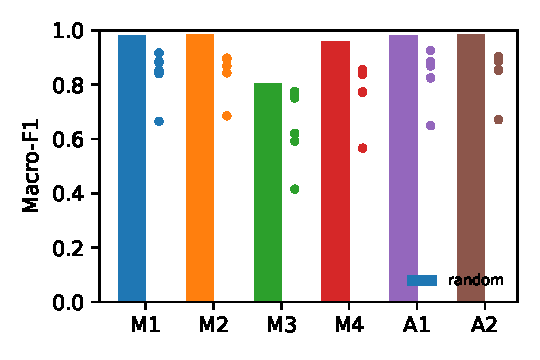
\includegraphics[width=\columnwidth]{figures/random_vs_source_disjoint.pdf}
\caption{Random-split versus source-disjoint macro-F1 per model. Markers are individual holdouts.}
\label{fig:vs}
\end{figure}

\begin{figure}[!htbp]
\centering
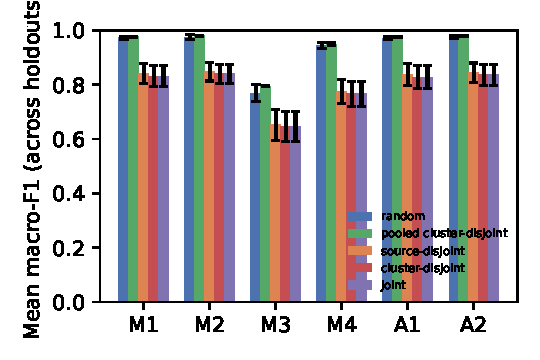
\includegraphics[width=\columnwidth]{figures/protocol_comparison.pdf}
\caption{Mean macro-F1 by protocol and model across the six holdouts. Error bars are standard errors across holdouts.}
\label{fig:protocol}
\end{figure}

\begin{figure}[!htbp]
\centering
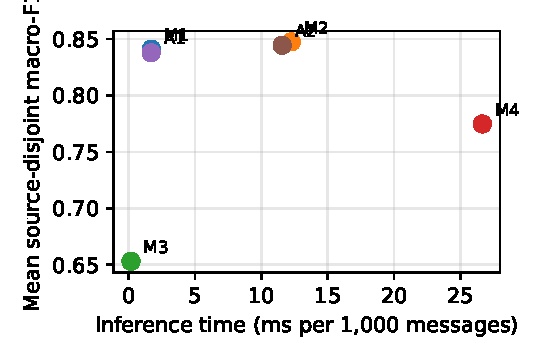
\includegraphics[width=\columnwidth]{figures/accuracy_efficiency_tradeoff.pdf}
\caption{Source-disjoint mean macro-F1 against per-1000 inference time.}
\label{fig:eff}
\end{figure}

Table~\ref{tab:performance_summary} summarises the headline numbers by design. On the primary random split, \RandomBestModel{} reached a macro-F1 of \RandomBestMacroFOne{} (95\% CI \RandomBestMacroFOneCI), the highest of the six models. Under source-disjoint evaluation, \SourceBestModel{} achieved the highest macro-F1 at \SourceBestMacroFOne{} (95\% CI \SourceBestMacroFOneCI). The best-of-best generalisation gap is \GeneralisationGap{}; this single number, however, conceals substantial per-model and per-holdout variation.

Table~\ref{tab:per_model_gap} reports the per-model generalisation gap (random-split macro-F1 minus source-disjoint macro-F1) with mean, median, range, worst case, paired-bootstrap 95\% CI, and Wilcoxon signed-rank $p$ across the six holdouts. The mean gap ranges from \GapMeanMTwo{} (M2) to \GapMeanMFour{} (M4); the worst-case holdout gap reaches \GapWorstMFour{} (M4). All six models show a positive mean gap with a Wilcoxon $p$ of \WilcoxonP{}. This $p$-value is the two-sided floor for $n=6$ when all signs agree: it confirms that the direction of the drop is consistent across holdouts for every model, but it is not independent per-model evidence, because the six holdouts are shared across models.

% Generated by deceptive-email manuscript.py
% run_id: 20260811T162016Z_d2881b85
% timestamp_utc: 2026-08-12T21:16:26Z
% source_artifact: outputs/runs/<run_id>/metrics/paired_delta.csv

\begin{table*}[!htbp]
\centering
\caption{Per-model generalisation gap (random-split macro-F1 minus source-disjoint macro-F1) across the six holdouts. CI is a paired bootstrap 95\% interval over 1{,}000 replicates; Wilcoxon p is the signed-rank test across holdouts.}
\label{tab:per_model_gap}
\begin{tabular}{lcccccc}
\hline\hline
Model & Mean & Median & Min & Max & 95\% CI & $p$ \\
\hline
M2 & 0.138 & 0.105 & 0.088 & 0.300 & [0.094, 0.208] & 0.031 \\
A2 & 0.139 & 0.114 & 0.081 & 0.313 & [0.092, 0.213] & 0.031 \\
M3 & 0.151 & 0.118 & 0.029 & 0.388 & [0.062, 0.266] & 0.031 \\
M1 & 0.141 & 0.114 & 0.065 & 0.317 & [0.089, 0.219] & 0.031 \\
A1 & 0.143 & 0.111 & 0.055 & 0.332 & [0.087, 0.226] & 0.031 \\
M4 & 0.184 & 0.153 & 0.103 & 0.392 & [0.122, 0.277] & 0.031 \\
\hline\hline
\end{tabular}
\end{table*}


Across the six source-disjoint holdouts (Tables~\ref{tab:holdout} and~\ref{tab:performance_summary}; full per-split detail in Table~S1 of \texttt{supplementary.tex} in the replication repository), the mean macro-F1 was \SourceMeanMacroFOneMOne{} for M1, \SourceMeanMacroFOneMTwo{} for M2, \SourceMeanMacroFOneMThree{} for M3, \SourceMeanMacroFOneMFour{} for M4, \SourceMeanMacroFOneAOne{} for A1, and \SourceMeanMacroFOneATwo{} for A2. The structural model M3 degraded substantially from the random split to every source-disjoint holdout; its mean source-disjoint macro-F1 of \SourceMeanMacroFOneMThree{} trails every other model by a wide margin. The gradient-boosted tree M4 also drops more than the linear text models; its mean source-disjoint macro-F1 of \SourceMeanMacroFOneMFour{} is the second-lowest. The linear text models (M1, M2, A1, A2) form a tight cluster around \SourceMeanMacroFOneMOne{}--\SourceMeanMacroFOneATwo{}. The no-anonymization-token ablations A1 and A2 track M1 and M2 closely, indicating that the bracketed tokens are not a primary discriminative shortcut for the linear text models.

Table~\ref{tab:cluster_leakage} quantifies the near-duplicate leakage each protocol permits. On four of six holdouts, source-disjoint splits still contain tens to hundreds of thousands of cross-split exact-SimHash pairs (e.g., 518,677 for the trec6+trec7 holdout); on the remaining two holdouts (trec5 and trec5+trec6) the count is zero. Because every source sits entirely on one side of a source-disjoint split, every surviving cross-split pair is necessarily cross-source: a training row from one source reproduces a test row from a different source. What source separation removes is therefore within-source replication, and what it leaves is cross-source template replication. The cluster-disjoint and joint protocols eliminate these pairs by construction. The random full-match controls contain 198,199--690,608 cross-split pairs, confirming that random splits exploit both within-source and cross-source replication.

Table~\ref{tab:decomposition} reports the decomposition analyses. The source-predictability probe shows that the training features encode source identity with \SourcePredMin{}--\SourcePredMax{} cross-validated accuracy on the two-source training partitions (chance 0.5), confirming that source artefacts are highly learnable. The PSI ranges from \PSIMin{} to \PSIMax{} and the KS statistic from \KSMin{} to \KSMax{}, indicating substantial train/test distribution shift on the most demanding holdouts. The OOV share ranges from \OOVMin{} to \OOVMax{}, so 12--17\% of test tokens are absent from the training vocabulary. Training-only threshold recalibration changes macro-F1 by at most \RecalMaxGain{} (on the trec5+trec6 holdout) and by small or negative amounts elsewhere, so the F1 drop is dominated by discrimination loss rather than calibration drift.

% Generated by deceptive-email manuscript.py
% run_id: 20260811T162016Z_d2881b85
% timestamp_utc: 2026-08-12T21:16:26Z
% source_artifact: outputs/runs/<run_id>/metrics/distribution_divergence.csv

\begin{table*}[!htbp]
\centering
\caption{Decomposition of the source-disjoint drop. Source predictability is the 3-fold CV accuracy of a source classifier on the training partition (chance 0.5 for two-source training). PSI and KS quantify train/test TF-IDF divergence; OOV is the test-token share absent from the training vocabulary; recalibration gain is the mean macro-F1 change from training-only isotonic threshold recalibration across probabilistic models.}
\label{tab:decomposition}
\begin{tabular}{lcccccc}
\hline\hline
Holdout & Source pred. & PSI & KS & OOV share & Recal. gain \\
\hline
trec5 & 0.961 & 0.359 & 0.243 & 0.116 & +0.012 \\
trec5|trec6 & -- & 0.377 & 0.242 & 0.128 & +0.053 \\
trec5|trec7 & -- & 0.116 & 0.138 & 0.147 & +0.001 \\
trec6 & 0.965 & 0.035 & 0.046 & 0.154 & +0.003 \\
trec6|trec7 & -- & 0.145 & 0.106 & 0.169 & -0.015 \\
trec7 & 0.955 & 0.149 & 0.109 & 0.158 & -0.019 \\
\hline\hline
\end{tabular}
\end{table*}


Table~\ref{tab:paired_delta} reports the paired macro-F1 delta (random minus protocol) per model per protocol with paired-bootstrap CIs and Cohen's $d$. The cluster-disjoint and joint protocols produce deltas very close to the source-disjoint deltas, because the cluster rule removes only the within-source replication that the source rule already removes for cross-source pairs; the remaining gap is dominated by genuine source shift rather than by near-duplicate leakage. The sources-pooled cluster-disjoint protocol isolates the template-replication component: its mean delta is only \PooledClusterGapMean{} (range \PooledClusterGapMin{}--\PooledClusterGapMax{}) across models, an order of magnitude smaller than the source-disjoint deltas. Template replication alone therefore inflates random-split macro-F1 by only a few thousandths, whereas source shift accounts for the bulk of the \GapMeanMTwo{}--\GapMeanMFour{} drop.

% Generated by deceptive-email manuscript.py
% run_id: 20260811T162016Z_d2881b85
% timestamp_utc: 2026-08-12T21:16:26Z
% source_artifact: outputs/runs/<run_id>/metrics/paired_delta.csv
% Edited for page-limit compliance: cluster-disjoint and joint source
% cluster-disjoint rows removed (values are essentially identical to
% source-disjoint because the cluster rule is subsumed by the source
% rule on source-disjoint splits; their mean paired delta is within
% 0.01 of source-disjoint).

\begin{table*}[!htbp]
\centering
\caption{Paired macro-F1 delta (random minus protocol) per model across the six holdouts. SD = source-disjoint; RCD-p = sources-pooled cluster-disjoint (no source held out). CI is a paired bootstrap 95\% interval over 1{,}000 replicates; $p$ is the Wilcoxon signed-rank test across holdouts. The RCD-p delta isolates template replication without source shift.}
\label{tab:paired_delta}
\begin{tabular}{llccccc}
\hline\hline
Model & Protocol & Mean $\Delta$ & Median & 95\% CI & Cohen's $d$ & $p$ \\
\hline
M2 & SD       & 0.138 & 0.105 & [0.094, 0.208] & 1.69 & 0.031 \\
A2 & SD       & 0.139 & 0.114 & [0.092, 0.213] & 1.59 & 0.031 \\
M3 & SD       & 0.151 & 0.118 & [0.062, 0.266] & 1.08 & 0.031 \\
M1 & SD       & 0.141 & 0.114 & [0.089, 0.219] & 1.57 & 0.031 \\
A1 & SD       & 0.143 & 0.111 & [0.087, 0.226] & 1.47 & 0.031 \\
M4 & SD       & 0.184 & 0.153 & [0.122, 0.277] & 1.70 & 0.031 \\
M2 & RCD-p     & 0.005 & 0.004 & [0.002, 0.008] & 1.15 & 0.031 \\
A2 & RCD-p     & 0.004 & 0.002 & [0.001, 0.007] & 0.89 & 0.031 \\
M3 & RCD-p     & 0.009 & 0.006 & [0.004, 0.013] & 1.32 & 0.031 \\
M1 & RCD-p     & 0.006 & 0.005 & [0.003, 0.009] & 1.42 & 0.031 \\
A1 & RCD-p     & 0.006 & 0.006 & [0.003, 0.009] & 1.53 & 0.031 \\
M4 & RCD-p     & 0.009 & 0.006 & [0.002, 0.017] & 0.89 & 0.062 \\
\hline\hline
\end{tabular}
\end{table*}

The near-duplicate analysis found \NExactDupGroups{} identical-SimHash groups covering \NExactDupRows{} rows, of which \NExactDupCrossGroups{} cross-source groups contain \NExactDupCrossRows{} rows.

The rank-based and calibration metrics preserve discrimination more than macro-F1. On the six source-disjoint holdouts, M1 retains ROC-AUC above \MOneROCaucMinNoDigit{} on every holdout while its macro-F1 falls to \MOneFOneTrecNoDigit{} on the trec5+trec6 holdout. This is consistent with the cross-model observation of Gutierrez et al.~\cite{gutierrez_crossmodel_2026} that discrimination ranking is largely preserved across source shift. The Brier diagnostic, however, shows that the F1 drop is not primarily a calibration artifact: training-only isotonic recalibration recovers at most \RecalMaxGain{} macro-F1 (Table~\ref{tab:decomposition}), and the Brier scores on the most demanding holdouts (\MOneBrierTrecNoDigit{}--\MFourBrierTrecNoDigit{} for M1/M4 on trec5+trec6) indicate genuine miscalibration that threshold adjustment alone cannot remove. Brier is unavailable for the linear SVMs (M2, A2), which do not produce calibrated probabilities.

Fig.~\ref{fig:vs} compares the random-split macro-F1 of each model with its per-holdout source-disjoint macro-F1. Fig.~\ref{fig:protocol} compares the mean macro-F1 across the five protocols. The per-model generalisation gap is shown numerically in Table~\ref{tab:per_model_gap}.

All pairwise McNemar comparisons between the structurally distinct model families (M1/M2 vs M3 vs M4) were significant at the Holm-corrected level on every split tested (\texttt{outputs/runs/20260811T162016Z\_d2881b85/\\metrics/model\_comparisons.csv}: 215 of 225 pairwise tests significant at $\alpha=\McNemarAlpha$ after Holm correction; the ten non-significant tests involve near-duplicate model pairs such as M1 vs A1, M2 vs A2, or A1 vs A2, which differ only in whether anonymization tokens are stripped). The original M1 versus M2 contrast was significant on every split. We caution, however, that statistical significance does not imply a stable model ordering across holdouts: the per-holdout rankings in Table~\ref{tab:holdout} show that the best model varies with the held-out source, so we do not claim that any model is best across all holdouts.

\subsection{Independent-corpus validation}
To test whether the models' cross-source behaviour transfers beyond the three TREC sources, we evaluated the same six models on an independent corpus: the ealvaradob/phishing-dataset texts subset (20,069 messages after cleaning, 7,660 positive and 12,409 benign), which is derived from Enron employee mail plus phishing samples and is temporally and institutionally distinct from the TREC spam tracks. The exact-text overlap with the cleaned MeAJOR corpus is zero, and only 41 of 20,069 secondary SimHash values collide with primary SimHash values, so the two corpora are effectively disjoint at the content level. Models trained on the MeAJOR random-split training partition achieve macro-F1 of \SecFMOne{} (M1), \SecFMTwo{} (M2), \SecFMThree{} (M3), \SecFMFour{} (M4), \SecFAOne{} (A1), and \SecFATwo{} (A2) on the secondary corpus. The linear text models retain most of their discrimination, the structural model M3 collapses (macro-F1 \SecFMThree{}, MCC \SecMThreeMCC{}, worse than chance), and the gradient-boosted tree M4 drops to \SecFMFour{}. This pattern mirrors the source-disjoint results on MeAJOR. We caution that this is a model-portability check, not a validation of the leakage-resistant protocol itself: the models were trained on the MeAJOR random-split partition, and the secondary corpus mixes Enron ham with phishing samples whose label semantics differ from the TREC spam-track positive class, so the two corpora are not label-compatible benchmarks.

\section{Discussion}
The evaluation protocol changes the measured performance of every model, and the magnitude depends on the model and the held-out source. Under random splitting the best macro-F1 is \RandomBestMacroFOne{}; under source-disjoint evaluation the best is \SourceBestMacroFOne{}. The per-model mean gap ranges from \GapMeanMTwo{} (M2) to \GapMeanMFour{} (M4), with worst-case \GapWorstMFour{}, consistent with dataset shift~\cite{dataset_shift}: a random split lets a model rely on near-duplicate campaigns that a source-disjoint holdout removes.

The decomposition analyses separate the contributing effects. The source-predictability probe (\SourcePredMin{}--\SourcePredMax{} CV accuracy) shows the features encode source identity; PSI and KS show substantial train/test shift on demanding holdouts; the OOV share (12--17\%) shows unseen test vocabulary; training-only recalibration recovers at most \RecalMaxGain{}, so the F1 drop is dominated by discrimination loss rather than calibration drift. Source separation alone is not sufficient: on four of six holdouts, source-disjoint splits still contain 40,705--518,677 cross-split exact-SimHash pairs, all cross-source. The sources-pooled cluster-disjoint protocol isolates the template component: a mean delta of only \PooledClusterGapMean{} shows template replication alone inflates random-split macro-F1 by only a few thousandths, whereas source shift accounts for the bulk of the \GapMeanMTwo{}--\GapMeanMFour{} drop.

The four linear text models (M1, M2, A1, A2) form a tight cluster with mean source-disjoint macro-F1 between \SourceMeanMacroFOneMOne{} and \SourceMeanMacroFOneATwo{}; ablations A1/A2 track M1/M2, so the bracketed tokens are not a primary discriminative shortcut. The gradient-boosted tree M4 drops more steeply than the linear text models (\SourceMeanMacroFOneMFour{}), consistent with over-fitting to within-source token statistics. The structural model M3 collapses (\SourceMeanMacroFOneMThree{}), suggesting that the URL, attachment, and language features encode source-specific statistics rather than a portable signal; this is mirrored by M3's collapse to macro-F1 \SecFMThree{} on the secondary corpus while the linear text models retain 0.86--0.90. These are observational findings for three sources, not causal claims about feature families.

On efficiency, M1 and A1 offer the strongest accuracy-to-cost trade; they trail M2 and A2 by a small margin on source-disjoint mean macro-F1 while costing a fraction of the inference time. M2 and A2 are the most accurate under both protocols but are the most expensive, and M3 is cheapest and weakest. M4 sits between the linear text models and M3 in both axes. Fig.~\ref{fig:eff} visualises this trade-off.

Our conclusions are limited to the three source corpora in the cleaned MeAJOR release, the independent secondary corpus, and the models we evaluated. We do not claim deployment readiness, and the dataset's positive class should be read as the MeAJOR labels rather than an independent ground truth. Future work should extend the protocol to additional corpora, temporal splits, and multilingual settings.

\section{Conclusion}
We proposed a reusable, leakage-resistant evaluation protocol for cross-source deceptive-email detection and applied it to the MeAJOR corpus (\NDocs{} records, \NSources{} sources). Across \NSplits{} splits and six lightweight models, random splits inflate measured macro-F1 by a per-model mean of \MeanGeneralisationGap{} (range \GapMeanMTwo{}--\GapMeanMFour{}); source separation alone is necessary but not sufficient to prevent campaign or template leakage; and the F1 drop is dominated by genuine discrimination loss rather than calibration drift. The sources-pooled cluster-disjoint control isolates source shift as the dominant mechanism (template replication alone inflates macro-F1 by only \PooledClusterGapMean{}). We release the protocol, split manifests, SimHash parameters, and reproduction commands.

\section*{Reproducibility}
A versioned reproducibility manifest is bundled with this submission at \texttt{outputs/package/20260811T162016Z\_d2881b85\_\\reproducibility\_manifest.zip} (see \texttt{reports/reproducibility.md}). The manifest records SHA-256 checksums for all prediction sets, metrics, fitted models, split manifests, configuration, and source-tree hash, together with the SimHash parameters (64-bit, 4 bands $\times$ 16 bits, exact at Hamming 0, near-duplicates at $\le 8$), the cluster-disjoint rule, and the matched-control construction. The replication repository, which also contains the supplementary file \texttt{supplementary.tex} (Table~S1), is publicly available at \url{https://github.com/Weihang-Huang/DeceptionEmail}; reproduction commands are in \texttt{reports/reproducibility.md}. \textbf{A persistent Zenodo DOI for the replication repository will be added before final submission; reviewers requiring access to the camera-ready artifacts may contact the corresponding author.}

\section*{Acknowledgment}
The authors thank the developers of the open-source software used in this study: scikit-learn~\cite{sklearn}, LIBLINEAR~\cite{liblinear}, and the XGBoost~\cite{chen_xgboost} library. No external funding was received for this work.

\bibliographystyle{IEEEtran}
\bibliography{references}

\end{document}
